\documentclass[11pt]{kiseon_memo}

\title{Monte Carlo simulation of stochastically heated grains
       and comparison with the Guhathakurta--Draine method}
\author{Kwang-il Seon}
\date{\today}

\usepackage{amsmath, amssymb}
\usepackage{siunitx}
\usepackage{booktabs}
\usepackage{tabularx}
\usepackage{graphicx}
\usepackage[round,authoryear]{natbib}
\usepackage{microtype}
\usepackage{hyperref}
\usepackage[section]{placeins}    % \FloatBarrier at every \section
% Allow LaTeX more flexibility avoiding overfull boxes in body text.
\sloppy

\newcommand{\Cabs}{C_{\rm abs}}
\newcommand{\Qabs}{Q_{\rm abs}}
\newcommand{\QplT}{\langle Q_{\rm abs} \rangle_T}
\newcommand{\Ctot}{C_{\rm tot}}
\newcommand{\Cvol}{C_{\rm vol}}
\newcommand{\Teq}{T_{\rm eq}}
\newcommand{\umc}{\,\mu{\rm m}}
\newcommand{\ulam}{u_\lambda}
\newcommand{\Jlam}{J_\lambda}
\newcommand{\sigmaSB}{\sigma_{\rm SB}}
\newcommand{\Bnu}{B_\nu}
\newcommand{\Blam}{B_\lambda}
\newcommand{\evt}{N_{\rm evt}}

\begin{document}
\maketitle

\begin{abstract}
We implement the Monte Carlo (MC) algorithm of
\citet{DraineAnderson1985} for tracking the temperature of a single
interstellar dust grain through individual photon-absorption events,
extend it with a selectable heat-capacity backend, and reproduce
Figures~24.5 and 24.6 of \citet{DrainePIIM2011}.  The standalone
implementation is kept for visualization; a subroutine-form API is
then used to integrate $P(T)$ over a grain size distribution and
build an emergent SED.  The SED builder exposes a runtime flag
\texttt{use\_mc\_for\_large\_grain}.  In the default mode
($\texttt{=\,F}$), small (stochastic) grains use the Monte Carlo
engine while large (equilibrium) grains use the analytic
\texttt{calc\_Teq} solver -- the same hybrid logic the production
pipeline uses, but with MC replacing the
\citet{GuhathakurtaDraine1989} matrix solver in the stochastic
branch.  In this mode the MC-based SED reproduces the production
\texttt{sed\_solve} output to within $1$--$3\%$ in every band, once
three corrections are applied to the SED builder: (i) a
fractional-temperature cap on the linearized cooling step, which keeps
the super-linear $T^4$ cooling from over-populating the hot tail of
$P(T)$ (otherwise a $\sim 20\%$ mid-IR over-prediction for the tiniest
PAHs); (ii) a single-grain energy-conservation rescale that forces each
grain's grey bolometric emission to equal its absorbed power, removing
a Planck-midpoint convexity bias; and (iii) charge-resolved PAH
emission (neutral and cation summed separately, as the production
solver does), which fixes a $\sim 23\%$ near-IR deficit.  Setting the
flag to \texttt{T} switches large grains to MC as well.  The all-MC
mode additionally needs an adaptive cutoff
$\lambda_c(a) = hc / (\delta T_{\rm thresh}\,\Teq\,\Ctot(\Teq))$
(\S\ref{sec:adaptive_lamc}) in place of the static
$\lambda_c=1000\,\mu$m: without it the single-photon temperature jumps for
large grains are too small to keep the trajectory near $\Teq$ and the
FIR is under-predicted by $\sim 30\%$.  With all corrections the all-MC
SED is indistinguishable from the default mode (both within $1$--$3\%$
of the reference) and the single-grain $T_{\rm rad}^{\rm MC}/\Teq$ ratio
stays within $\pm 3\%$ across $a \in [0.03, 5]\,\mu$m.  A second
runtime flag,
\texttt{mc\_engine}, selects between the original fixed-grid histogram
(log $[2,5000]$~K, $N_{\rm hist}=600$) and two adaptive-grid engines
introduced in Section~\ref{sec:adaptive}: a deterministic two-pass
engine that probes $T_{\rm min}/T_{\rm max}$ in a first pass and replays
the trajectory with the same RNG state on a fitted grid, and a single-
pass engine that buffers sub-step samples and bins them after the run.
Both adaptive engines auto-select log versus linear spacing based on
$T_{\rm max}/T_{\rm min}$, which gives a $\sim 50\times$ sharper
resolution of the narrow equilibrium $P(T)$ for large grains where the
fixed grid collapses to one populated bin. \emph{All Monte Carlo results
in this report (Figures~\ref{fig:fig245}--\ref{fig:pT_large}) use the
adaptive two-pass engine}; the fixed-grid engine is retained in the code
for backward compatibility and is shown only as a baseline in
Figure~\ref{fig:pT_large}.
\end{abstract}

\paragraph{Note on the Mathis ISRF.} The production
\texttt{radfield.f90 :: J\_Mathis}, which mc\_pT shares with
\texttt{sed\_solve}, was switched on 2026-05-17 to the
Draine's corrected 4000\,K dilution factor ($1.65\times 10^{-13}$,
Draine textbook 2011 Table~12.1; the literal Mathis~1983 $10^{-13}$
value used previously is retained as
\texttt{use\_mathis\_corrected = .false.} for reproducibility, with
full discussion in
\texttt{SEDust/docs/astrodust\_sed\_report.tex} \S7.1.1,
``Mathis 4000\,K dilution correction''). At the fiducial
$a=0.1\umc$ astrodust grain the correction shifts $T_{\rm eq}$ by
$+0.22$\,K ($+1.28\%$) and the FIR-peak emission per grain by
$+8.4\%$. The PIIM Figs.~24.5/24.6 reproductions
(Figures~\ref{fig:fig245}, \ref{fig:fig246}), the SED comparison
against \texttt{sed\_solve} (Figure~\ref{fig:sed_compare}), and the
single-grain $P(T)$ comparisons (Figures~\ref{fig:pT_ad},
\ref{fig:pT_pah}, \ref{fig:pT_large}) have all been regenerated with
the new default and the adaptive two-pass MC engine; the $1$--$3\%$
MC-vs-reference agreement is invariant to the choice of dilution
factor because both sides shift together.

\tableofcontents

\section{Introduction}

A dust grain in the interstellar medium absorbs starlight photons
discretely.  When the grain is macroscopic ($a \gtrsim 0.03\umc$),
many absorption events occur per radiative cooling time and the grain
sits at a well-defined equilibrium temperature $\Teq(a)$ at which the
mean absorbed power balances the radiative cooling.  Smaller grains,
however, do not have enough heat capacity to absorb the energy of a
single starlight photon without making a large, transient excursion
in temperature.  Each photon absorption raises the grain's
temperature by tens to hundreds of Kelvin; between events the grain
cools radiatively back toward $\Teq$.  The temperature history $T(t)$
is a sequence of sharp upward spikes followed by long, slow exponential
cooling tails, as illustrated in Figure~24.5 of \citet{DrainePIIM2011}.

Because the emission spectrum scales steeply with temperature
($\propto T^4$ in total luminosity, with strong wavelength
dependence through the Planck function and the cross section),
the spectral energy distribution (SED) of small grains is dominated
by the high-temperature spikes, not by $\Teq$.  Quantitative treatment
requires the probability distribution $P(T)$, which is the fraction
of time the grain spends at each temperature in steady state.

There are two standard ways to obtain $P(T)$:
\begin{enumerate}
\item \textbf{Monte Carlo} \citep{DraineAnderson1985}.  Simulate the
  stochastic sequence of absorption events directly and accumulate a
  time-weighted histogram of $T(t)$.
\item \textbf{Discretized steady-state matrix solve}
  \citep{GuhathakurtaDraine1989, DraineLi2001}.  Discretize $T$ into
  bins, build a transition matrix from absorption (upward) and
  Planck-averaged emission (downward) rates, and solve for the steady
  state.
\end{enumerate}
The matrix method is more efficient and is what the production
astrodust pipeline uses (\texttt{p\_sub.f90::calc\_P}).  The MC method
is conceptually simpler, has fewer numerical knobs, and provides a
useful independent cross-check.  This document records the MC
implementation kept under \verb|SEDust/mc/| and its validation.

\paragraph{Document layout.}
Section~\ref{sec:algo} derives the MC algorithm and the cooling ODE
used between events.  Section~\ref{sec:impl} describes the Fortran
module structure and the selectable heat-capacity backend.
Section~\ref{sec:valid} presents the reproduction of
\citet{DrainePIIM2011} Figures~24.5 and~24.6 and the energy-balance
test.  Section~\ref{sec:sed} describes the subroutine-form API and
the SED builder that integrates $P(T)$ over a grain size distribution.
Section~\ref{sec:compare} compares the MC-based SED against the
Guhathakurta--Draine matrix solver on identical inputs.

\section{Algorithm}\label{sec:algo}

\subsection{Two-regime treatment of the absorbed radiation field}

Consider a spherical grain of radius $a$ in an isotropic radiation
field of mean intensity $\Jlam(\lambda)$.  The radiative energy
density per unit wavelength is
\begin{equation}
\ulam = \frac{4\pi}{c}\Jlam \quad
[\text{erg}\,\text{cm}^{-3}\,\umc^{-1}].
\end{equation}
The grain absorbs photons of wavelength $\lambda$ at a rate per unit
wavelength
\begin{equation}\label{eq:dRate}
\frac{dN_{\rm abs}}{dt\,d\lambda}
   = \pi a^2 \, \Qabs(a,\lambda)\,\frac{c\,\ulam\,\lambda}{hc}
   = \frac{\pi a^2}{h}\,\Qabs(a,\lambda)\,\ulam\,\lambda,
\end{equation}
where the photon energy is $E = hc/\lambda$ and we have used
$\ulam/E = (\ulam\,\lambda)/(hc)$ as the photon number density per
unit wavelength, multiplied by $c$ to get a photon flux density and
by $\pi a^2\,\Qabs$ to get the absorption rate.

\citet{DraineAnderson1985} split this rate into a continuous part
(long wavelengths, where photons arrive so frequently that the grain
heat content increases smoothly) and a stochastic part (short
wavelengths, where individual events are resolved).  Pick a cutoff
$\lambda_c$ (default $1000\umc$).  The continuous-heating rate per
unit surface area is
\begin{equation}\label{eq:Hcont}
H(a) \;\equiv\; \frac{c}{4}\!\int_{\lambda_c}^{\infty}\!
       \Qabs(a,\lambda)\,\ulam\,d\lambda
       \quad [{\rm erg}\,{\rm cm}^{-2}\,{\rm s}^{-1}].
\end{equation}
The stochastic event rate is
\begin{equation}\label{eq:rateEvt}
\Gamma_{\rm evt}(a) \;\equiv\;
       \int_{0}^{\lambda_c}\!
       \frac{dN_{\rm abs}}{dt\,d\lambda}\,d\lambda
       \quad [{\rm s}^{-1}].
\end{equation}
For the Mathis ISRF and a small grain, $\Gamma_{\rm evt}$ is dominated
by ultraviolet photons; $H(a)$ is essentially the CMB contribution and
is numerically negligible.  Both contributions are nevertheless kept
so that the same code handles dense-cloud and starlight-heated
conditions uniformly.

The tabulated wavelength grid generally has one interval straddling
$\lambda_c$.  That interval is split at $\lambda_c$ by linear
interpolation of the integrand: its blueward part is added to
$\Gamma_{\rm evt}$ (and to the photon-sampling CDF) and its redward
part to $H(a)$, so the cutoff bin is dropped from neither term.  The
sampling CDF is built from the same split integral as
$\Gamma_{\rm evt}$ and has its last node pinned at $\lambda_c$, so a
sampled photon always satisfies $\lambda \le \lambda_c$.  A grain with
no absorption blueward of $\lambda_c$ has $\Gamma_{\rm evt}=0$ and
belongs on the equilibrium path; \texttt{grain\_setup\_from\_cabs}
stops with a diagnostic rather than divide by a zero event rate.

\subsection{Cooling ODE between events}

Let $E_{\rm grain}(T)$ be the total grain enthalpy and
$\Ctot(T) \equiv dE_{\rm grain}/dT$ its total heat capacity.  Between
absorption events, the grain's energy evolves according to
\begin{equation}
\frac{dE_{\rm grain}}{dt} = P_{\rm heat} - P_{\rm emit}
   = 4\pi a^2 \bigl[\,H(a) - \QplT \sigmaSB T^4\,\bigr],
\end{equation}
where $\QplT$ is the Planck-averaged absorption efficiency,
\begin{equation}\label{eq:Qpl}
\QplT \;\equiv\;
   \frac{\int \Qabs(a,\lambda)\,\Blam(T)\,d\lambda}
        {\int \Blam(T)\,d\lambda}.
\end{equation}
Dividing through by $\Ctot$ gives the cooling ODE used in the MC:
\begin{equation}\label{eq:cooling}
\boxed{\;\frac{dT}{dt}
   = \frac{4\pi a^2}{\Ctot(T)}\,
     \bigl[\,H(a) - \QplT\,\sigmaSB\,T^4\,\bigr].\;}
\end{equation}
Equation~(\ref{eq:cooling}) is identical to Eq.~(2.9) of
\citet{DraineAnderson1985}, which writes it in the equivalent form
$dT/dt = (3/(a\,\Cvol(T)))\,(H - \QplT\sigmaSB T^4)$ using the heat
capacity per unit volume $\Cvol = \Ctot/(4\pi a^3/3)$.  We use the
total form because the enthalpy routine
(\texttt{SED\_v5/enthalpy\_v2.f90::enthalpy\_DL01}) returns the total
grain enthalpy in erg.  The factor $4\pi a^2$ in our form is the
grain \emph{surface} area (heating and emission are surface effects),
and the $1/\Ctot$ absorbs the grain volume implicit in the total
heat capacity.

\subsection{The Monte Carlo loop}

Starting from $(t_0, T_0)$, one step of the MC simulation does the
following.

\begin{enumerate}
\item\textbf{Sample the inter-arrival time.}
  The event-arrival process is Poissonian with rate
  $\Gamma_{\rm evt}$, so the waiting time
  $\Delta t = -\ln U_1 / \Gamma_{\rm evt}$
  where $U_1 \in (0,1]$ is a uniform random number.
\item\textbf{Integrate Eq.~(\ref{eq:cooling}) over $[t_0, t_0+\Delta t]$.}
  The grain cools (or, in the rare regime where $H > \QplT\sigmaSB T^4$,
  heats) according to the continuous part of the radiation field.
  During this step we accumulate the time-weighted contribution to the
  $P(T)$ histogram and to the integrated emitted energy.
\item\textbf{Sample the absorbed photon.}
  Choose a wavelength $\lambda$ from the normalized PDF
  $p(\lambda) \propto dN_{\rm abs}/(dt\,d\lambda)$ on
  $(0,\lambda_c)$, via inverse-CDF lookup on a pre-tabulated CDF.
\item\textbf{Apply the enthalpy jump.}
  The absorbed photon energy $E_{\rm phot} = hc/\lambda$ goes into
  internal vibrational energy.  Solve
  \begin{equation}\label{eq:jump}
  E_{\rm grain}(T_{\rm after}) = E_{\rm grain}(T_{\rm before})
                                + E_{\rm phot}
  \end{equation}
  for $T_{\rm after}$ by inverting the tabulated $E_{\rm grain}(T)$.
\end{enumerate}

The loop is repeated for a prescribed total number $\evt$ of events
(typical: $10^4$--$5\times10^4$ per grain for good $P(T)$ statistics),
or until a prescribed total simulated time is reached.

\subsection{Integrator for the cooling ODE}

For a typical $\sim100\,\textrm{\AA}$ graphite grain in $U=1$
starlight, the inter-arrival time is $\Delta t \sim 600\,$s while the
radiative cooling time after a photon spike is $\sim$~ms.  The cooling
ODE~(\ref{eq:cooling}) is therefore mildly stiff: rapid initial decay
followed by a long, near-equilibrium tail.  Explicit Euler is
prohibitively slow because the step size near equilibrium is set by
the restoring rate, which is large.

Substantively the right-hand side of Eq.~(\ref{eq:cooling}) is
dominated, after the photon spike, by the $T^4$ Stefan--Boltzmann
emission term: with $H(a)\ll \QplT \sigmaSB T^4$ the equation reduces
to $dT/dt \simeq -(4\pi a^2/\Ctot)\QplT\sigmaSB T^4$.  Both $\Ctot(T)$
(Debye) and $\QplT$ are weakly $T$-dependent, so the trajectory is
not a single exponential -- it falls steeply at high $T$ and slowly
near $\Teq$.  Any closed-form fit (exponential, power-law $T^{-3}$
from constant-$C$ Stefan--Boltzmann) is an approximation; we therefore
integrate Eq.~(\ref{eq:cooling}) numerically and, when a continuous
$T(t)$ is needed for a figure, dump the actual integrator sub-step
samples rather than reconstructing from event boundaries.

We use a linearly-implicit (exponential) step.  At the current
temperature $T_0$, we form a one-sided finite difference to estimate
the local slope
\begin{equation}
\Lambda(T_0) \;\equiv\; \frac{d(dT/dt)}{dT}\bigg|_{T_0}
   \approx \frac{(dT/dt)_{1.01\,T_0} - (dT/dt)_{T_0}}{0.01\,T_0}.
\end{equation}
When $\Lambda < 0$ the dynamics is locally a stable relaxation
toward a local equilibrium temperature
$T_{\rm eq, loc} = T_0 - (dT/dt)_{T_0}/\Lambda$, and the linearized
solution
\begin{equation}\label{eq:expstep}
T(t_0 + dt) \;=\; T_{\rm eq, loc} +
   \bigl(T_0 - T_{\rm eq, loc}\bigr)\,e^{\Lambda \, dt}
\end{equation}
is exact.  We step by
\begin{equation}\label{eq:stepcap}
dt = \min\!\Bigl(dt_{\rm left},\; \tfrac{\ln 2}{|\Lambda|},\;
     f_{\rm cap}\,\tfrac{T_0}{|dT/dt|_{T_0}}\Bigr),
     \qquad f_{\rm cap} = 0.05,
\end{equation}
once $|T_0 - T_{\rm eq, loc}|/T_0 < 10^{-3}$ we take the full
remaining $dt_{\rm left}$ in a single step, since further evolution is
unobservable on the bin scale.  The first cap, $\ln 2 / |\Lambda|$,
halves the distance to local equilibrium per step.  The third cap,
which limits the \emph{fractional} temperature change to
$f_{\rm cap}=5\%$ per step, is essential: the linearized
solution~(\ref{eq:expstep}) is exact only for a locally
\emph{linear} ODE, whereas the true cooling is strongly super-linear
($dT/dt \propto -\QplT T^4$).  Over a half-life-sized step the local
linearization lags the faster early cooling, so the grain appears to
linger at high $T$, over-populating the hot tail of $P(T)$ and
over-emitting in the mid-IR.  This bias is most severe for the
violently heated tiniest PAH grains and was the dominant source of an
MC mid-IR over-prediction before the $f_{\rm cap}$ cap was added
(\S\ref{sec:charge_rescale}).  With the cap, the
linearization error per step is negligible; the step count per cooling segment
is bounded by a hard cap (\texttt{MAX\_STEPS} $=4000$ in the fixed-grid
\texttt{cool\_segment}, $300$ in the adaptive engines of
\S\ref{sec:adaptive}).

The $P(T)$ histogram and the emitted-energy bookkeeping sub-sample each
step at $N_{\rm sub}=8$ interior points of the sub-step trajectory,
each carrying weight $dt/N_{\rm sub}$, so a step that spans several
histogram bins deposits its time weight across all of them.
For unstable ($\Lambda \ge 0$) or degenerate cases the fallback is a
forward Euler step, also subject to the $f_{\rm cap}$ cap.

\section{Implementation}\label{sec:impl}

\subsection{Module layout}

The implementation lives under \verb|SEDust/mc/| and is split
into small modules that each do one thing.  Throughout, cgs units
are used (erg, cm, s) except that wavelength is in $\umc$ to match
the rest of the astrodust pipeline.

\begin{itemize}
\item \verb|mc_heatcap.f90|: enthalpy $E_{\rm grain}(T,a)$ and heat
  capacity $\Ctot(T)=dE_{\rm grain}/dT$ for selectable compositions
  (Table~\ref{tab:hc}).  $\Ctot$ is computed by central differences on
  $E_{\rm grain}$, which works for all backends without composition-specific
  analytic derivatives.

\item \verb|mc_rng.f90|: thread-local pseudo-random number generator
  (\textsf{xorshift64*}, period $2^{64}-1$) wrapped in a derived type
  \verb|rng_t|.  Each OpenMP thread owns its own state, so no locking
  is needed inside the MC inner loop.

\item \verb|mc_grain_type.f90|: derived type \verb|mc_grain_t| holding
  all single-grain pre-tabulated state ($\lambda$ grid, $\Qabs$, $\ulam$,
  $H_{\rm cont}$, $\Gamma_{\rm evt}$, photon-wavelength CDF, $T$ grid,
  $E_{\rm grain}(T)$, $\QplT$).  Instances are local to a thread.

\item \verb|mc_engine.f90|: the engine.  Two setup entry points:
  \verb|grain_setup_graphite| (D16 graphite sphere Q, used by the
  standalone validation path) and \verb|grain_setup_from_cabs|
  (arbitrary $\Cabs(\lambda)$, used by the SED builder).  Three MC
  drivers with the same signature shape, differing only in the
  histogram strategy:
  \verb|mc_run_engine| (the original fixed-grid log $[2, 5000]$~K
  histogram),
  \verb|mc_run_engine_2pass|, and
  \verb|mc_run_engine_buffered|.  All three return the time-weighted
  $P(T)$ histogram (as bin edges $T_{\rm edge}$, $dP/dT$, and
  $dP/d\ln T$) and the integrated absorbed and emitted energies; the
  adaptive engines additionally return the auto-selected grid type
  (\texttt{is\_log\_out}) and the observed $T_{\rm min}/T_{\rm max}$.
  Common helpers --- \verb|step_advance|, \verb|sub_sample_step|,
  \verb|build_adaptive_grid|, \verb|bin_sub_samples| --- factor out the
  trajectory math and the log/linear binning so each driver is short
  and the integrator code is shared.  See
  Section~\ref{sec:adaptive} for the algorithm and rationale.

\item \verb|mc_sed.f90|: SED builder.  Wraps an OpenMP parallel-do
  loop over the size distribution; each iteration creates its own
  \verb|mc_grain_t| and \verb|rng_t|, runs MC, and accumulates the
  thread-local contribution to $\lambda I_\lambda$.

\item \verb|main_mc.f90|: standalone single-grain driver
  (\verb|main_mc.x|).  Reads a namelist, runs one MC, writes
  \verb|<prefix>_PT.dat|.

\item \verb|main_mc_sed.f90|: size-distribution SED driver
  (\verb|main_mc_sed.x|).  Reads a namelist, calls \verb|sed_init|
  from the astrodust pipeline to load the grain Q table, size
  distribution, and PAH cross sections, then loops via \verb|mc_sed|.
\end{itemize}

\begin{table}[ht]
\centering
\caption{Selectable heat-capacity backends (\texttt{comp} key).}
\label{tab:hc}
\begin{tabularx}{\linewidth}{lX}
\toprule
key & enthalpy model \\
\midrule
\texttt{gra\_dl01} & DL01 \texttt{Car0} graphite (Debye-2 with $\Theta_1=863$ K, $\Theta_2=2504$ K, plus CH modes for $n_{\rm atom}<10^4$).  \textbf{Default for graphite and PAH.} \\
\texttt{gra\_d85}  & Single Debye-3, $\Theta_D=420$ K, $n_{\rm atom}=1.14\times10^{23}$ cm$^{-3}$.  Original \citet{DraineAnderson1985} prescription. \\
\texttt{sil\_dl01} & DL01 silicate (\texttt{Sil}). \\
\texttt{ad\_s1\_c1} & Astrodust Stage 1, C1 prefactor (pure DL01 \texttt{Sil}). \\
\texttt{ad\_s1\_c2} & Astrodust Stage 1, C2 prefactor (density-corrected). \\
\texttt{ad\_s2}    & Astrodust Stage 2: $E_{\rm Sil}(N_{\rm Sil})+E_{\rm Car}(N_{\rm Car})$ via volume-weighted sub-volumes ($f_C^{\rm vol}=0.193$, $P=0.20$). \\
\bottomrule
\end{tabularx}
\end{table}

\subsection{Validation: energy conservation}

For each MC run we accumulate the absorbed energy $E_{\rm abs}=\sum_{\rm
events} hc/\lambda$ and the emitted energy
$E_{\rm emit} = \int 4\pi a^2 \QplT \sigmaSB T^4\,dt$ over the full
simulation.  In steady state these should match.  The standalone
\verb|main_mc.x| (adaptive two-pass engine) with $a=100$\AA{} graphite,
$U=1$, $N_{\rm evt}=2\times10^5$ returns $E_{\rm emit}/E_{\rm abs}=
0.997$ -- consistent with 1 within the residual from the finite final
state.  Larger grains, more events, and higher $U$ all push the ratio
closer to unity.

For the size-distribution SED builder (\verb|main_mc_sed.x|) on the
HD23 astrodust+PAH size distribution at $\log U=0.20$ ($U=1.585$), the
default-mode population-summed trajectory ratios are now
$E_{\rm emit}/E_{\rm abs} = 1.001$ (astrodust) and $1.000$ (PAH).  The
fractional-temperature step cap (Eq.~\ref{eq:stepcap}) removed the
$\sim 10\%$ deficit ($0.90$/$0.93$) that the uncapped linearized
integrator produced in earlier versions.  Independently of the raw
trajectory bookkeeping, the SED builder rescales each stochastically
heated grain's emission to its absorbed power
(\S\ref{sec:charge_rescale}), so the \emph{emitted SED} conserves
energy exactly by construction --- as the matrix solver does.  The
all-MC mode, where the large grains carry a small residual that this
rescale removes, is discussed in \S\ref{sec:energy_fix}.

\section{Validation against PIIM Figures 24.5 and 24.6}\label{sec:valid}

\subsection{Figure 24.5: $T(t)$ trajectories}

We run the standalone \verb|main_mc.x| with composition
\texttt{gra\_dl01} for the ten panels of \citet{DrainePIIM2011}
Figure~24.5: grain radii $\{10,20,50,100,200\}$\AA{} crossed with
$U\in\{1,10^2\}$. Each run is capped at $t_{\rm max}=10^5$~s
($\sim$1 day) following PIIM Fig.~24.5. The grain starts at
$T_{\rm init}=T_{\rm CMB}=2.725$~K (the code default, so the script
does not override it) and warms toward $\Teq$ on the first cooling
segment; the panels with $N_{\rm evt}=0$ (e.g.\ $a=10$\,\AA{} at
$U=1$, where no UV photon arrives within $t_{\rm max}$) therefore
sit on the cooling tail from $T_{\rm init}$ for the whole simulated
window. Total wall time across the 10 runs is $\sim 1.3$~s.

Figure~\ref{fig:fig245} reproduces the qualitative behavior of PIIM
Fig.~24.5: large grains ($a\geq 100$\AA) sit close to a steady
temperature; smaller grains spike to hundreds of K between sparse
photon events.  The energy balances in each panel are within $\sim 5\%$ for
all panels with $N_{\rm evt} > 100$.

\begin{figure}[ht]
\centering
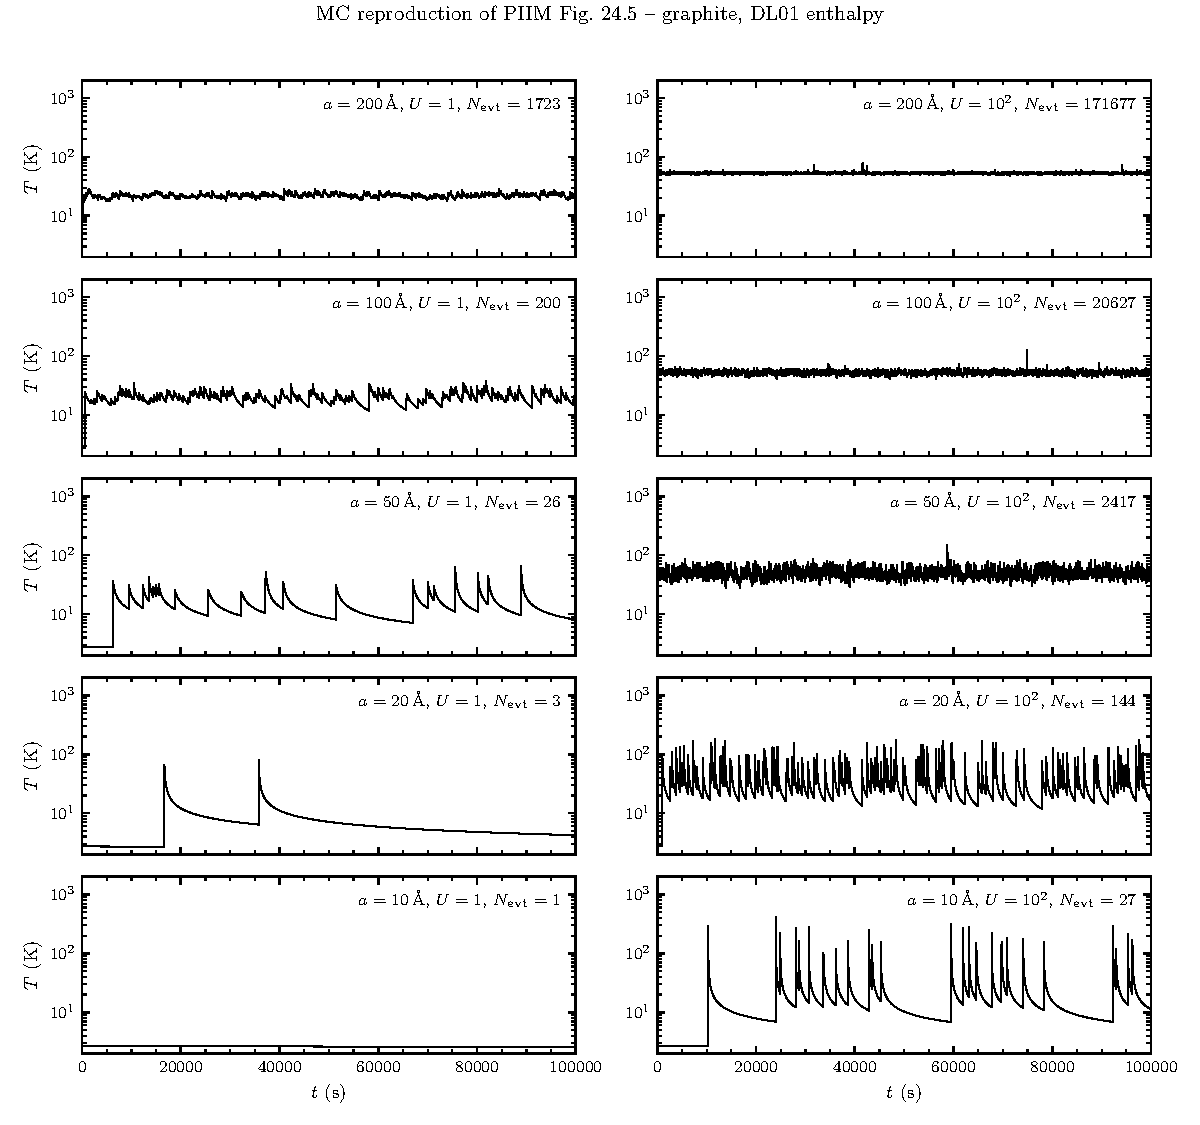
\includegraphics[width=\linewidth]{figs/fig24_5.pdf}
\caption{Reproduction of \citet{DrainePIIM2011} Figure~24.5: MC
  temperature histories for graphite grains in the local ISRF.
  Black curves are the actual cooling trajectories dumped from
  \texttt{cool\_segment} at the integrator's adaptive sub-step
  boundaries (no closed-form reconstruction); vertical line segments
  show the instantaneous photon-jumps from $T_{\rm pre}$ to
  $T_{\rm post}$ at each absorption event.}
\label{fig:fig245}
\end{figure}

\subsection{Figure 24.6: $dP/d\ln T$}

For the $P(T)$ reproduction we use the same five sizes at $U=1$ with
$N_{\rm evt}=2\times 10^4$ per grain.  Figure~\ref{fig:fig246} shows
the time-weighted $dP/d\ln T$ distributions, reproducing PIIM
Fig.~24.6: large grains have a narrow peak near $\Teq$; small grains
have broad distributions extending to several hundred K.

\begin{figure}[ht]
\centering
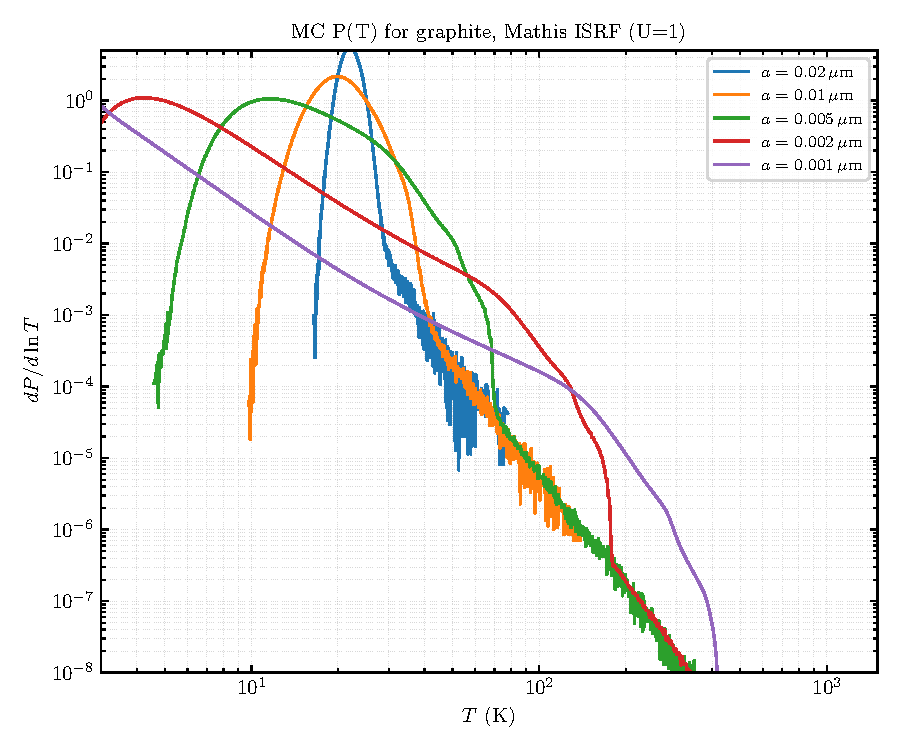
\includegraphics[width=0.75\linewidth]{figs/fig24_6.pdf}
\caption{$dP/d\ln T$ for graphite grains in the Mathis ISRF ($U=1$),
  for sizes $a\in\{0.001, 0.002, 0.005, 0.01, 0.02\}\umc$.  Compare
  with PIIM Figure~24.6.}
\label{fig:fig246}
\end{figure}

\section{SED builder over a grain size distribution}\label{sec:sed}

The \verb|mc_sed| module integrates $P(T)$ across the HD23 astrodust+PAH
size distribution (read by \verb|sed_astrodust_mod::sed_init| from
\verb|data/release/size_distribution.dat|) and produces the emission
SED $\lambda I_\lambda / N_H$ in the same units as the production
\verb|sed_solve| routine.

\subsection{SED accumulation}

For each grain $a_j$ in the size distribution:
\begin{equation}\label{eq:sed_sum}
J_\lambda \;+\!\!= \; (dn/N_H)_j \cdot \Cabs(\lambda, a_j) \cdot
   \sum_{i} \frac{w_i}{t_{\rm total}} \cdot \pi\,\Blam(T_{{\rm mid},i}),
\end{equation}
where $w_i$ is the time spent in histogram bin $i$ (with center
$T_{{\rm mid},i}$) accumulated by the MC.  Summing over both grain
populations (astrodust + PAH) and applying the same final unit
conversion as the production pipeline,
$\lambda I_\lambda = \lambda J_\lambda \times 10^{-3}$, gives the
final SED in erg s$^{-1}$ cm$^{-2}$ sr$^{-1}$ H$^{-1}$.

\subsection{Energy-conservation rescale and charge-resolved PAH}
\label{sec:charge_rescale}

Two refinements to the raw accumulation~(\ref{eq:sed_sum}) are needed
to bring the MC SED into band-by-band agreement with the matrix
solver.  Both were identified by isolating the residual to the PAH
component (the astrodust component agreed to $\sim 0.4\%$ from the
start) during the cross-check of Section~\ref{sec:compare}.

\paragraph{Single-grain energy-conservation rescale.}
Equation~(\ref{eq:sed_sum}) re-evaluates the Planck function at each
bin \emph{midpoint} $T_{{\rm mid},i}$.  Because $\Blam(T)$ is convex in
$T$ (the bolometric emission scales as $T^4$), the midpoint value
exceeds the bin-averaged emission --- a Jensen-inequality bias that
over-weights the hot tail and leaves the grain emitting slightly more
than it absorbed.  In steady state a grain emits exactly what it
absorbs (Kirchhoff), and the matrix solver enforces this by
construction.  We restore it in the MC builder by rescaling each
stochastically heated grain's spectrum by
\begin{equation}\label{eq:ec_rescale}
s_{\rm ec} \;=\; \frac{P_{\rm abs}}{P_{\rm emit}^{\rm grey}}, \qquad
P_{\rm emit}^{\rm grey} = \sum_i w_i\, 4\pi a^2 \QplT[T_{{\rm mid},i}]
   \sigmaSB T_{{\rm mid},i}^4, \qquad
P_{\rm abs} = \frac{E_{\rm abs}^{\rm evt}}{t_{\rm total}}
   + 4\pi a^2 H_{\rm cont},
\end{equation}
where $P_{\rm abs}$ is the grain's total absorbed power (discrete
photon events plus the continuous long-wavelength heating
$H_{\rm cont}$) and $P_{\rm emit}^{\rm grey}$ is the grey bolometric
emission of the same histogram.  The rescaled single-grain spectrum
$s_{\rm ec}\,J_\lambda^{(j)}$ then conserves energy exactly while
keeping the spectral \emph{shape} set by $P(T)$.  Combined with the
integrator step cap (\S\ref{sec:algo}, Eq.~\ref{eq:stepcap}), this
brought the integrated PAH power from $1.15\times$ the matrix-solver
reference (raw midpoint histogram, half-life step) to $1.005\times$.

\paragraph{Charge-resolved PAH populations.}
The production pipeline treats PAHs as a blend of two charge states,
neutral and cation, mixed by an ionization fraction $f_{\rm ion}(a)$;
the two have markedly different cross sections in the near-IR (the
cation carries a \citet{Mattioda2005} NIR continuum that the neutral
lacks).  The matrix solver loops over both charge states --- each with
its own $\Cabs$ and size-distribution weight $dn$ --- and sums the
emission.  The MC builder must do the same: \verb|mc_sed_solve_pah|
runs the engine twice per size, once with the neutral
$(\Cabs^{\rm neu}, dn^{\rm neu})$ and once with the cation
$(\Cabs^{\rm ion}, dn^{\rm ion})$ at an offset RNG seed, and sums.
Using the single charge-averaged cross section instead --- as an
earlier version did --- biases the PAH near-IR (1--5\,$\mu$m) low by
$\sim 23\%$.  Resolving the charge states moves the PAH NIR band ratio
from $0.77$ to $0.97$ relative to the reference.

\subsection{OpenMP parallelism}

The grain loop in \verb|mc_sed::mc_sed_loop| carries an
\texttt{!\$omp parallel do schedule(dynamic,1)} directive.  Each thread
holds its own \verb|mc_grain_t| and \verb|rng_t| in private storage and
contributes to a thread-local \verb|Jout_local(:)|; thread-local totals
are merged into the shared accumulator inside a single
\texttt{!\$omp critical} block at the end of the parallel region.

On a 12-core M-series Mac with $N_{\rm evt}=5\times 10^4$ per grain,
the population sum over $\sim 168$ grains (84 sizes $\times$ 2
populations) takes $\sim 14$~s wall time, about $11\times$ the
single-thread cost -- the slight loss versus the 12$\times$ ideal is
the cost of the dynamic schedule with variable work per grain.

\section{Comparison with the Guhathakurta--Draine matrix solver}\label{sec:compare}

We compare \verb|main_mc_sed.x| against the production astrodust
pipeline \verb|main_astrodust.x|.  Both implementations read the
same Q table (\verb|q_astrodust_P0.20_Fe0.00_1.400.dat|), the same
size distribution (HD23 \verb|size_distribution.dat|), the same
Mathis ISRF at $\log U=0.20$, and the same Stage 2 astrodust
enthalpy.

\subsection{Two solver modes}

The \verb|main_mc_sed.x| driver exposes a runtime namelist flag,
\verb|use_mc_for_large_grain|.  Small (stochastic) grains \emph{always}
use the Monte Carlo engine; the flag selects how large (equilibrium)
grains are handled:
\begin{itemize}
\item \texttt{use\_mc\_for\_large\_grain = .false.} (default).  Each grain
  is first tested with the equilibrium gate
  $E_{\rm grain}(\Teq)\ge 150$~eV (same threshold as
  \texttt{sed\_solve}).  Grains passing the gate are emitted as a
  delta-function at $\Teq$ via \texttt{calc\_Teq}.  Grains failing
  the gate are simulated with MC.
\item \texttt{use\_mc\_for\_large\_grain = .true.}  All grains use MC,
  regardless of size.  This exercises the MC engine on grains where
  the analytic solver is exact and exposes the integrator bias
  discussed below.
\end{itemize}

\begin{figure}[ht]
\centering
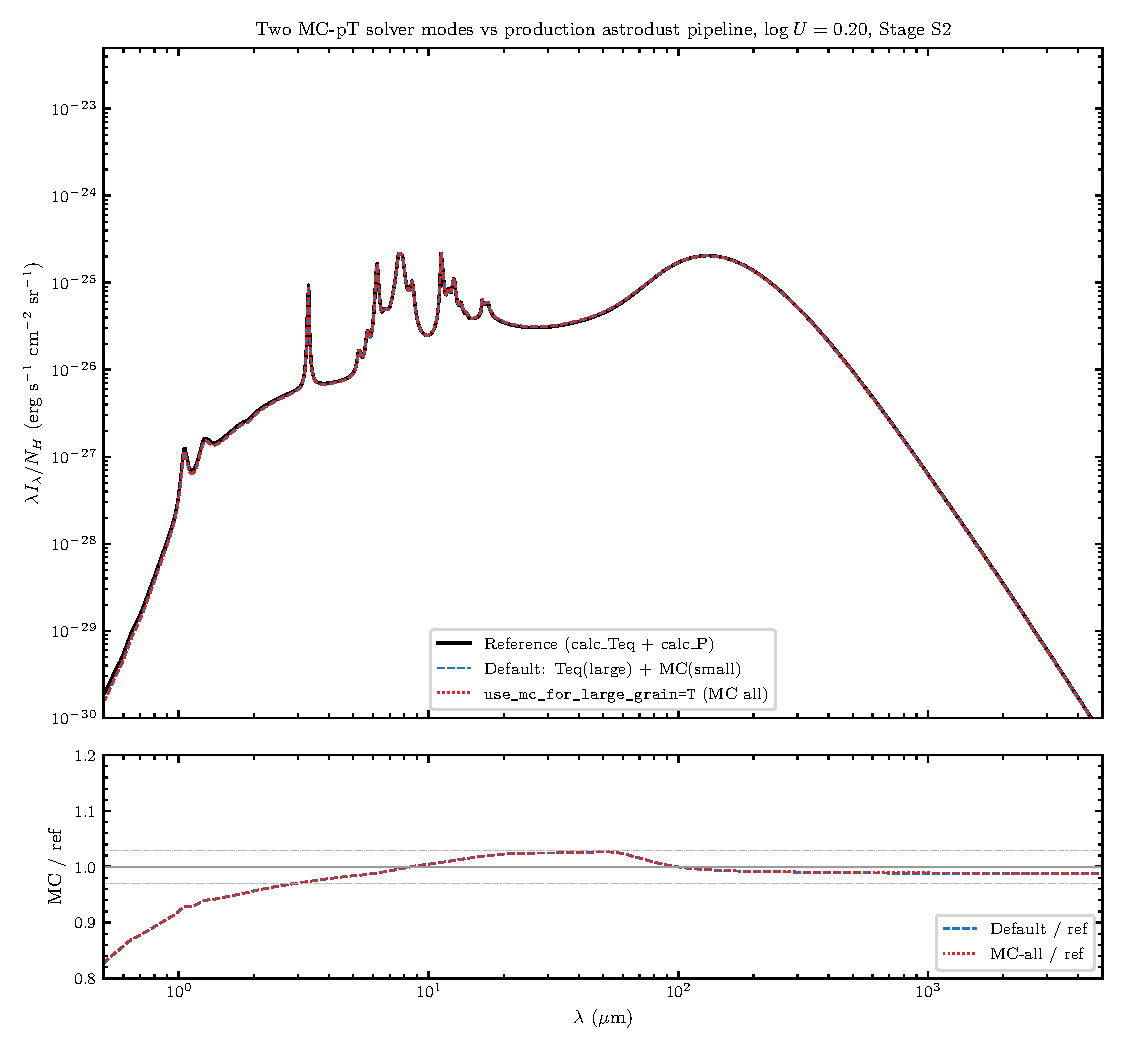
\includegraphics[width=\linewidth]{figs/sed_mc_vs_ref.pdf}
\caption{Two MC-pT solver modes versus the production astrodust
  pipeline, for the HD23 astrodust+PAH model in the Mathis ISRF at
  $\log U=0.20$, Stage 2 enthalpy. Both modes use the adaptive 2pass
  histogram engine, the integrator step cap (\S\ref{sec:algo}), the
  single-grain energy-conservation rescale and charge-resolved PAH
  (\S\ref{sec:charge_rescale}), and the adaptive
  \citet{DraineAnderson1985} cutoff
  $\lambda_c(a) = hc / (\delta T_{\rm thresh}\,\Teq\,C(\Teq))$ with
  $\delta T_{\rm thresh} = 0.01$ (\S\ref{sec:adaptive_lamc}).
  Top: $\lambda I_\lambda/N_H$. Bottom: ratio of each mode to the
  reference (note the expanded $0.8$--$1.2$ vertical scale). The
  default mode (blue dashed) and the all-MC mode (red dotted) are
  indistinguishable and both match the reference to within $1$--$3\%$
  in every band (NIR $0.97$, MIR $1.01$, FIR $1.00$, sub-mm $0.99$);
  the dip below $1\,\mu$m is at the optical/far-NIR edge, $\sim 5$
  decades below the peak and carrying negligible power. The
  $\sim 30\%$ all-MC FIR underprediction of earlier versions --- from
  large-grain trajectory collapse under a static
  $\lambda_c=1000\,\mu$m and from hot-tail over-population by the
  uncapped integrator --- is fully removed.}
\label{fig:sed_compare}
\end{figure}

Figure~\ref{fig:sed_compare} shows both modes against the reference.
In the default mode, MC handles 78 stochastic grains and
\texttt{calc\_Teq} handles 89 equilibrium grains (out of 167 total
across the two populations); the resulting SED matches the
production \texttt{sed\_solve} output to within $1$--$3\%$ in every
band.  In the \verb|use_mc_for_large_grain=T| mode, all 167 grains go
through MC and --- with the integrator and SED-builder fixes described
below --- the SED is essentially identical to the default mode
(band ratios agree to $< 0.5\%$ between the two modes).  This was not
the case in earlier versions, where the all-MC mode underpredicted the
FIR peak by $\sim 30\%$; the next subsection traces that bias and the
three changes that removed it.

\subsection{Energy conservation: the integrator and SED-builder
corrections}\label{sec:energy_fix}

The $\sim 30\%$ all-MC FIR deficit of earlier versions came from three
distinct biases, two opposite in sign, which a naive MC SED builder
incurs and which the production matrix solver does not.  Tracing them
required a component-by-component, band-by-band comparison (the astrodust component
agreed from the start; the residual was localized to PAH and to the
large equilibrium grains).

\begin{enumerate}
\item\textbf{Large-grain trajectory collapse (under-emission).}
  With the static cutoff $\lambda_c = 1000\,\mu$m, every photon a large
  grain absorbs is treated as a discrete event; but a large grain's
  heat capacity is so high that even a UV photon raises $T$ by
  $\ll \Teq$, so between events the trajectory relaxes toward the
  equilibrium of the \emph{continuous} heating alone (essentially
  $T_{\rm CMB}$) rather than toward $\Teq$.  The grain then radiates
  far too little.  This is the dominant part of the FIR deficit and is
  removed by the adaptive cutoff $\lambda_c(a)$ of
  \S\ref{sec:adaptive_lamc}, which folds the weak photons into the
  continuous term so the trajectory equilibrates at the correct
  $\Teq$.
\item\textbf{Hot-tail over-population (over-emission).}
  The linearized exponential step (\S\ref{sec:algo}) is exact only for
  a locally linear ODE; over a half-life-sized step it lags the
  super-linear $T^4$ cooling and the grain lingers hot, over-populating
  the high-$T$ tail of $P(T)$.  For the violently heated tiniest PAHs
  this over-predicts the mid-IR by up to $\sim 20\%$.  The fractional
  step cap $f_{\rm cap}=0.05$ (Eq.~\ref{eq:stepcap}) removes it; with
  the cap the raw trajectory energy ratio is
  $E_{\rm emit}/E_{\rm abs} = 1.001$ (astrodust) and $1.000$ (PAH) in
  the default mode, compared with $0.90$/$0.93$ for the uncapped
  integrator.  (In the all-MC mode the raw ratio is $0.97$/$1.00$, the
  residual $\sim 3\%$ astrodust deficit coming from the large grains
  whose narrow trajectory the MC still slightly under-resolves; this
  residual is removed per grain by the rescale below.)
\item\textbf{Planck-midpoint convexity (residual over-emission).}
  Re-evaluating $\Blam$ at bin midpoints over-weights the hot tail by
  Jensen's inequality.  The single-grain energy-conservation rescale of
  \S\ref{sec:charge_rescale} (Eq.~\ref{eq:ec_rescale}) forces the grey
  bolometric emission to equal the absorbed power, exactly as the
  matrix solver does by construction, so the SED conserves energy
  regardless of the residual.
\end{enumerate}

With all three corrections (plus the charge-resolved PAH of
\S\ref{sec:charge_rescale}, which fixes the near-IR), the all-MC mode
reproduces the analytic-large-grain reference to the same $1$--$3\%$ as
the default mode (Figure~\ref{fig:sed_compare}).  The earlier
characterization of the all-MC bias as ``an inherent bias of the
linearized integrator'' was correct for the uncapped step but is no
longer the operating regime.

\subsection{When to use each mode}

\begin{description}
\item[Default (\texttt{F}).]  Use for production runs.  This is the
  intended workflow: the MC engine handles the stochastically heated
  small grains (where it is genuinely needed) and the cheap analytic
  $\Teq$ solver handles the equilibrium grains (where it is exact).
  Total wall time on 12 cores is comparable to \texttt{main\_astrodust.x}
  (single-threaded) and the result reproduces the production SED.
\item[All-MC (\texttt{T}).]  Now a valid cross-check rather than a
  diagnostic-only mode: with the corrections of
  \S\ref{sec:energy_fix} it reproduces the reference to the same
  $1$--$3\%$ as the default mode.  The default mode is still preferred
  for production only because it is cheaper --- the analytic $\Teq$
  solver replaces an MC trajectory for each of the $\sim 90$
  equilibrium grains at no loss of accuracy (those grains are
  genuinely single-temperature).  Use all-MC when an end-to-end MC
  result is wanted, e.g.\ to validate the equilibrium gate itself.
\end{description}

\subsection{Wall-time scaling}

On the 12-core M-series Mac with $N_{\rm evt}=5\times 10^4$ per grain,
the default mode takes $\sim 17$~s wall (78 MC grains $+$ 89 analytic).
The all-MC mode takes $\sim 19$~s (all 167 grains MC).  By
comparison, \verb|main_astrodust.x| (single-threaded) takes $\sim 10$~s.
At $N_{\rm evt}=10^4$ (still 1--2\% statistical precision at most
$\lambda$) the MC wall times drop to $\sim 4$--$5$~s.  These figures
predate the fractional step cap (Eq.~\ref{eq:stepcap}); bounding the
step to $5\%$ in $T$ raises the sub-step count per cooling segment,
which increases the small-grain MC cost by a model-dependent factor of
a few.  The adaptive engines that produce these SEDs keep
\texttt{MAX\_STEPS} $=300$ (the fixed-grid \texttt{cool\_segment} uses
$4000$); with the $5\%$ cap the measured truncation rate is negligible
(about $6$ of $9.4\times 10^5$ cooling segments, $0.0006\%$, over a
full size-distribution run), so $300$ remains safe.
The MC is therefore now noticeably more expensive
per stochastic grain, which is a further reason to keep the cheap
analytic $\Teq$ branch for equilibrium grains in production.

\subsection{Single-grain $P(T)$ cross-check}\label{sec:per_grain_pT}

As a direct single-grain check of the MC temperature distribution against
the matrix solver --- independent of the size-distribution integral ---
we run a dedicated driver \verb|main_pT_compare.x| that, for
a hand-picked set of grain sizes, calls all three MC engines
(\verb|mc_run_engine|, \verb|mc_run_engine_2pass|,
\verb|mc_run_engine_buffered|) \emph{and} \verb|calc_P| on the same
input ($\Cabs$, $J_\lambda$, enthalpy, kappCMB, $T$ grid) and writes
four $dP/d\ln T$ blocks side by side. Figures~\ref{fig:pT_ad} and
\ref{fig:pT_pah} below show the adaptive two-pass block; the fixed-grid
block agrees with it at the stochastic sizes shown here (its
degeneracy issues appear only at $a \gtrsim 80\,\textrm{\AA}$ and are
documented in Figure~\ref{fig:pT_large}). We use
$N_{\rm evt}=5\times 10^5$ events per grain, which gives smooth
MC curves at the $10^{-5}$ level of $dP/d\ln T$.

Figures~\ref{fig:pT_ad} and \ref{fig:pT_pah} show the comparison for
four stochastic-regime sizes of each population.  With the step-capped
integrator (\S\ref{sec:algo}) the MC and GD distributions overlap to
plot accuracy across the body \emph{and} the high-$T$ tail, over the
full range of grain sizes --- the slight tail suppression seen in
earlier (uncapped) versions is gone.  The only visible difference is
at the extreme cold end, where the adaptive MC grid begins at the
lowest temperature the trajectory actually reached while \verb|calc_P|
extends to the bottom of the fixed $T$ grid; that region carries
negligible weight.  Near the peak of each distribution (which
dominates the SED) MC and GD agree to within a few percent.

\begin{figure}[ht]
\centering
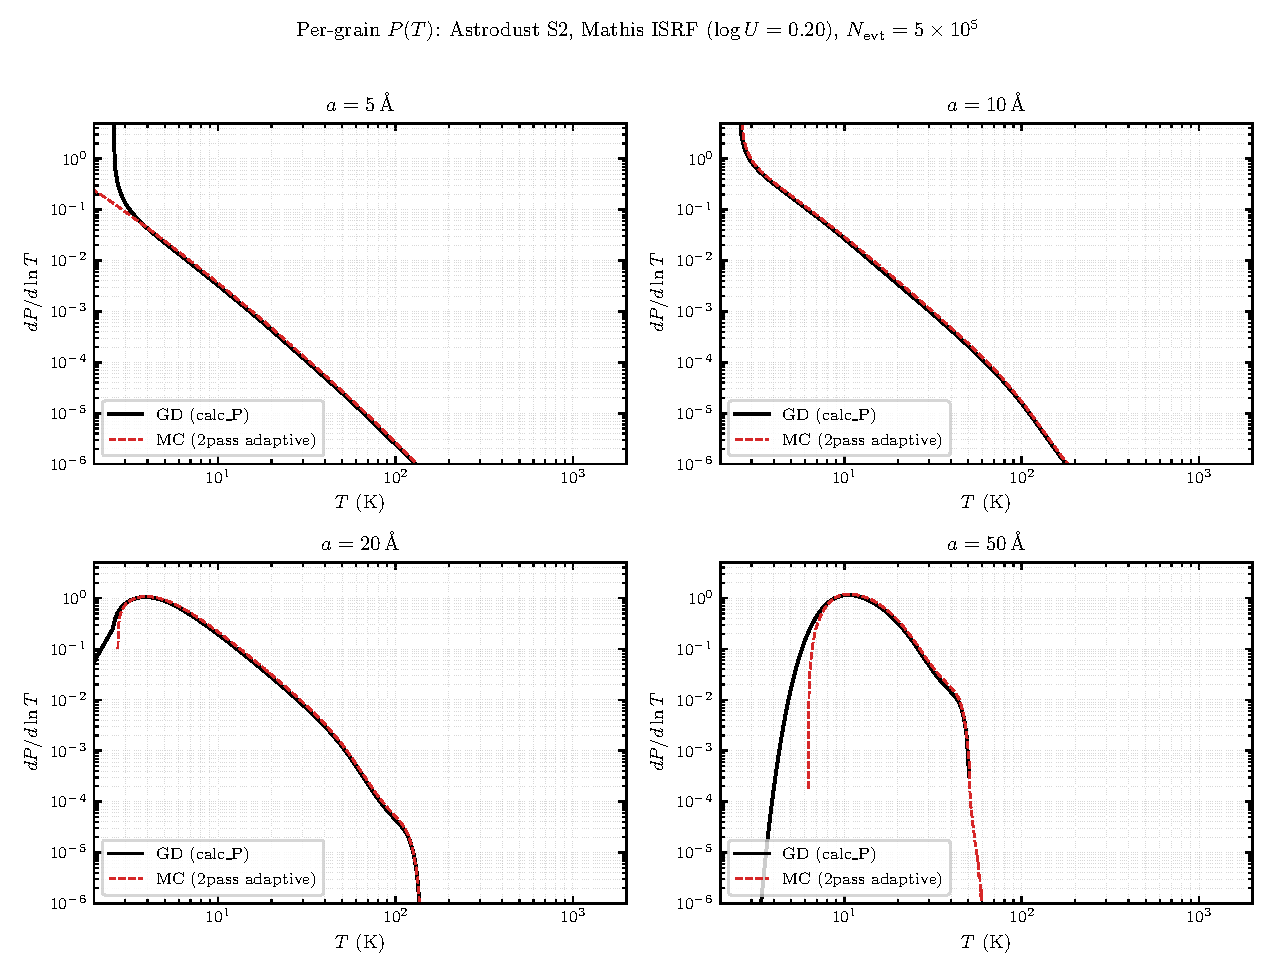
\includegraphics[width=\linewidth]{figs/pT_compare_astrodust.pdf}
\caption{Single-grain $dP/d\ln T$ for the astrodust population
  (Stage 2 enthalpy), four selected radii in the stochastic regime
  ($a = 5, 10, 20, 50\,\textrm{\AA}$).  Black: Guhathakurta--Draine
  matrix solver \texttt{calc\_P}.  Red dashed: Monte Carlo
  (\texttt{mc\_run\_engine\_2pass}, adaptive histogram grid,
  $N_{\rm evt}=5\times 10^5$).  The two solvers overlap on the body
  and the high-$T$ tail of each distribution; they differ only at the
  cold end, where the adaptive MC grid starts at the trajectory's
  observed minimum temperature.}
\label{fig:pT_ad}
\end{figure}

\begin{figure}[ht]
\centering
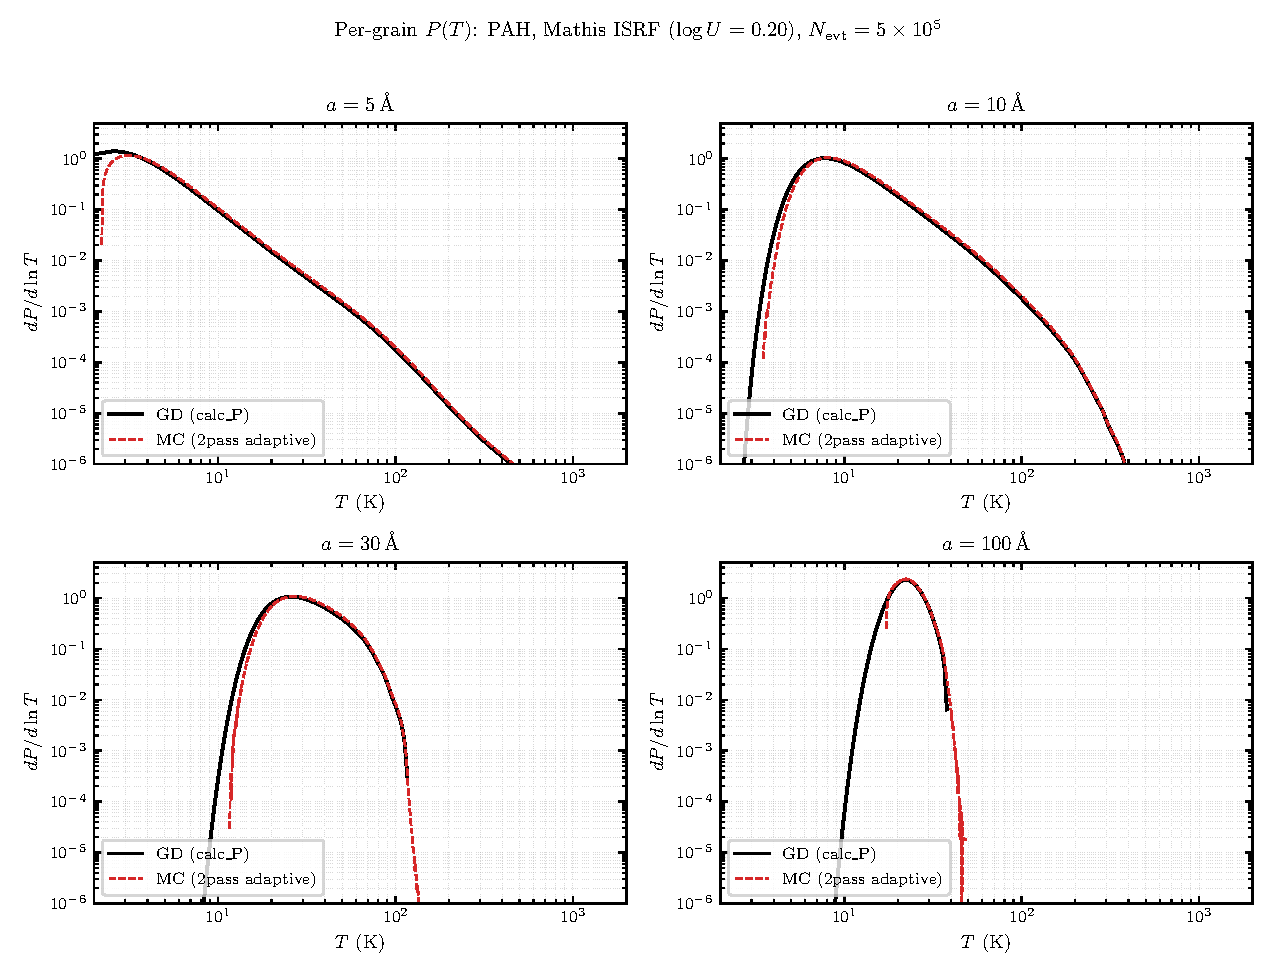
\includegraphics[width=\linewidth]{figs/pT_compare_pah.pdf}
\caption{Single-grain $dP/d\ln T$ for the PAH population, four selected
  radii ($a = 5, 10, 30, 100\,\textrm{\AA}$).  Same conventions as
  Fig.~\ref{fig:pT_ad} (adaptive two-pass MC engine, $N_{\rm evt}=
  5\times 10^5$).  At $a=5\,\textrm{\AA}$ the distribution extends to
  $\sim 400$~K, where MC and GD agree across five decades of
  $dP/d\ln T$.}
\label{fig:pT_pah}
\end{figure}

For equilibrium grains ($a \gtrsim 80\,\textrm{\AA}$ in the astrodust
population), the wide \verb|T_first| grid (1--3000~K, 250 log-spaced
bins) is too broad for \verb|calc_P| to resolve the narrow physical
$P(T)$ without the iterative narrowing logic used inside
\verb|sed_solve| (\verb|narrow_iterative| in
\verb|sed_astrodust.f90|).  Calling \verb|calc_P| directly returns
$P\equiv 0$ for these grains.  This is why our equilibrium-gate
branch in the default mode uses \verb|calc_Teq| (delta function at
$\Teq$) rather than \verb|calc_P| for them.  The adaptive two-pass MC
solver \emph{can} resolve the narrow $P(T)$ directly because it
builds the histogram grid from the observed
$(T_{\rm min}^{\rm obs}, T_{\rm max}^{\rm obs})$ of the trajectory
itself rather than from a pre-set wide range; see
Section~\ref{sec:adaptive} for the algorithm and Figure
\ref{fig:pT_large} for the resulting $\sim 50\times$ resolution gain
over the fixed-grid baseline.

\section{Adaptive-grid MC engines}\label{sec:adaptive}

The original engine \verb|mc_run_engine| uses a fixed log histogram on
$[T_{\rm min}, T_{\rm max}] = [2, 5000]\,$K with $N_{\rm hist}=600$
bins.  This is appropriate for the small (stochastic) grains for
which the algorithm was designed: the trajectory spans most of the
range and the log spacing matches the multi-decade nature of $P(T)$.
For large grains, however, the trajectory stays within a narrow
$(\Teq \pm \mathcal{O}(\sigma_T))$ band of width
$\Delta T/T \sim 1/\sqrt{E_{\rm grain}(\Teq)}$.  At $a=500\,\textrm{\AA}$
in the local ISRF the entire physical $P(T)$ fits inside
$[16.6, 19.5]\,$K, which is one bin of the fixed log grid.  The
histogram becomes a single populated bin at $T_{\rm mid}\approx \Teq$,
which is fine for the SED integral
(Eq.~\ref{eq:sed_sum}; the bin weight times $\Blam(T_{\rm mid})$
recovers the correct emission to better than $0.5\%$) but useless
as a diagnostic of the actual distribution shape.

To address this we add two adaptive-grid engines that build the
histogram grid from the observed trajectory itself.

\paragraph{Method A: two-pass with deterministic RNG replay
(\texttt{mc\_run\_engine\_2pass}).}
Pass~1 runs the MC trajectory exactly as in the original engine but
\emph{does not bin}; it only tracks the running
$(T_{\rm min}^{\rm obs}, T_{\rm max}^{\rm obs})$ across all sub-step
samples after a burn-in of $N_{\rm burn}=\max(50, N_{\rm pass1}/20)$
events (to exclude the initial $T_{\rm init}\to \Teq$ transient).
At the start of Pass~1 the RNG state is saved
(\texttt{rng\_saved = rng\%state}); at the end of Pass~1 the adaptive
grid is built from the observed range (with a $\pm 5\%$ margin) and
the RNG state is restored. Pass~2 re-runs the trajectory for the full
$N_{\rm evt}$ events. Because the integrator and the photon-sampling
routine are deterministic in their inputs and the RNG is restored to
bit-for-bit the same state, Pass~2 traces the identical path as Pass~1
and the only new work is binning. The cost is therefore
$\sim 2\times$ the fixed-grid engine. We expose \texttt{N\_pass1} as
an explicit argument but \emph{default to N\_pass1 = N\_events} (the
full trajectory) because shortening Pass~1 to a sub-trajectory makes
the adaptive grid built from $N_{\rm pass1} < N_{\rm evt}$ samples too
narrow: the remaining Pass~2 samples that fall outside the grid are
silently dropped by \texttt{bin\_sub\_samples} and the resulting
histogram weight sum drops below unity, biasing the SED low at the
FIR/sub-mm (the dropped tail samples are mostly at high $T$, whose
Rayleigh--Jeans-side flux at long $\lambda$ is linear in $T$).
Empirically, $N_{\rm pass1}=N_{\rm evt}/2$ produced an extra
$\sim 2$--$10$ percentage-point FIR/sub-mm deficit on top of the
integrator-bias deficit; reverting to the full Pass~1 closes that gap
to better than $1\%$ across the entire $0.1$--$3000\,\mu$m grid.

\paragraph{Method B: single-pass with sample buffer
(\texttt{mc\_run\_engine\_buffered}).}
The trajectory is integrated once.  Sub-step pairs $(T_{\rm sub}, dt_{\rm sub})$
after the burn-in are appended to caller-supplied arrays up to a
capacity $N_{\rm cap}$ (default $200\,000$ samples).  The running
$(T_{\rm min}^{\rm obs}, T_{\rm max}^{\rm obs})$ is tracked online and
is \emph{not} bounded by the capacity, so the adaptive grid built at
the end uses the true range of the simulated trajectory.  Binning
runs after the simulation completes.  If the buffer fills mid-run
(typical for very small grains and very large grains with many sub-
steps per cool segment), only the first $N_{\rm cap}$ post-burn-in
samples enter the histogram.  In steady state this is statistically
unbiased; in practice it produces a $\sim 1\%$ NIR shift in the SED
relative to Method~A for the smallest grains.  Cost is $\sim$ the
same as the original engine.

\paragraph{Adaptive grid spacing.}
Both methods call \verb|build_adaptive_grid| with margin $\epsilon=0.05$:
\begin{equation}
T_{\rm lo} = (1-\epsilon)\,T_{\rm min}^{\rm obs}, \quad
T_{\rm hi} = (1+\epsilon)\,T_{\rm max}^{\rm obs}.
\end{equation}
If $T_{\rm hi}/T_{\rm lo} > 3$, the bins are log-spaced from $T_{\rm lo}$
to $T_{\rm hi}$; otherwise they are linearly spaced.  The threshold
captures the qualitative split between multi-decade stochastic excursions
(where log is natural and resolves the high-$T$ tail) and narrow Teq
distributions (where linear gives bins of uniform $\Delta T$
matched to $\sigma_T$).  For the case in
Fig.~\ref{fig:pT_large}, the four shown grains span both regimes:
$a=100\,\textrm{\AA}$ picks log (range $[8.4, 35.8]\,$K, ratio $4.3$);
$a=200$, $501$, $1000\,\textrm{\AA}$ pick linear (ratios $1.84$,
$1.17$, $1.04$).  The bin lookup is $O(1)$ in both cases.

\paragraph{Runtime selection.}
\verb|main_mc_sed.x| exposes a namelist key \verb|mc_engine|
$\in\{$\texttt{'fixed'}, \texttt{'2pass'}, \texttt{'buffered'}$\}$
that dispatches grain by grain inside the OpenMP loop. The
default is \texttt{'2pass'} (adaptive). The \texttt{'fixed'} engine
is unsafe whenever \verb|use_mc_for_large_grain=.true.| because its
single populated bin in the equilibrium regime carries no diagnostic
content; the driver detects this combination at startup and
auto-promotes the engine to \texttt{'2pass'} with a logged warning.
The SED outputs of the three engines agree to better than $0.5\%$ at
every wavelength: the histogram strategy affects $P(T)$ resolution but
not the integrated emission, because each bin's contribution is
$dP/dT\cdot \Delta T \cdot \Blam(T_{\rm mid})$ and the product of
weight and Planck function is insensitive to bin refinement once the
distribution is reasonably sampled.

\paragraph{Pass~1 vs Pass~2 length in \texttt{mc\_run\_engine\_2pass}.}
The first pass exists only to probe
$(T_{\rm min}^{\rm obs}, T_{\rm max}^{\rm obs})$; the routine accepts
an explicit \texttt{N\_pass1} argument but \emph{defaults to N\_events}
(full trajectory) because shortening Pass~1 to a sub-trajectory makes
the adaptive grid built from $N_{\rm pass1} < N_{\rm evt}$ samples too
narrow: Pass~2 samples that fall outside the grid are silently dropped
by \texttt{bin\_sub\_samples} and the histogram weight sum drops below
unity, biasing the SED low at the FIR/sub-mm. Reverting to the full
Pass~1 closes that gap to better than $1\%$ across the entire
$0.1$--$3000\,\mu$m grid.

\subsection{Adaptive DA85 cutoff $\lambda_c(a)$}\label{sec:adaptive_lamc}

The \citet{DraineAnderson1985} stochastic/continuous split (\S\ref{sec:algo})
treats photons with $\lambda > \lambda_c$ as a continuous heating
term $H(a)$ and photons with $\lambda < \lambda_c$ as individual
stochastic events that produce a temperature jump
$\delta T = (hc/\lambda) / \Ctot(T)$. The split is heuristic: it
assumes the individual jumps are large enough to be statistically
significant compared to a typical $\Teq$ fluctuation. A fixed cutoff
$\lambda_c=1000\,\mu$m, used in earlier versions of this code, is
the right scale for small ($a \lesssim 0.1\,\mu$m) astrodust grains
but becomes physically wrong for larger grains. As $a$ grows the
heat capacity $\Ctot \propto a^3$ grows fast enough that even
UV-photon jumps $\delta T \ll \Teq$, and the trajectory between
events relaxes toward the local equilibrium of $H_{\rm cont}$ alone
(essentially $T_{\rm CMB}$ for Mathis ISRF) rather than toward $\Teq$.
The result is the trajectory collapse documented in
Figure~\ref{fig:pT_large}'s middle--bottom rows (with the static
$\lambda_c$) and the $\sim 30\%$ FIR underprediction of the all-MC
SED.

We replace the static $\lambda_c$ with an adaptive prescription
implemented in \texttt{mc\_sed\_loop} and \texttt{main\_pT\_compare}:
\begin{equation}\label{eq:lamc_adapt}
\boxed{\lambda_c(a) \;=\; \frac{hc}{\delta T_{\rm thresh}\,\Teq(a)\,\Ctot\!\bigl(\Teq(a),\,a\bigr)},}
\end{equation}
with $\delta T_{\rm thresh} = 0.01$. Photons with $\lambda$ short
enough that their single-event jump exceeds $\delta T_{\rm thresh}\,\Teq$
are kept stochastic; everything longer is folded into $H_{\rm cont}$.
$\Teq(a)$ is supplied by \texttt{calc\_Teq} on the same single-grain
cross sections; $\Ctot$ is the grain heat capacity at $\Teq$.
$\lambda_c$ is clamped to the wavelength grid so the split integrals
have at least one bin on each side.

For a single $a$ the formula scales as
$\lambda_c(a) \propto 1/\Ctot \propto a^{-3}$, recovering the user's
ansatz $\lambda_c(a) = \lambda_{c,0} \cdot (a_{\rm ref}/a)^3$ with the
prefactor fixed by the physical threshold rather than by hand. For
the HD23 astrodust size distribution at $\log U = 0.20$ the result
is $\lambda_c \approx 1000\,\mu$m (clamp) for $a \lesssim 100\,\textrm{\AA}$
(no change from the legacy behaviour) and $\lambda_c \approx 0.09\,\mu$m
(also clamp, at the short-wavelength edge of the grid) for
$a \gtrsim 0.05\,\mu$m, meaning that for all equilibrium grains the
full continuous spectrum is folded into $H_{\rm cont}$ and
\texttt{cool\_segment} naturally relaxes to the true $\Teq$.

The single-grain diagnostic written by \texttt{mc\_sed\_loop} when
\texttt{use\_mc\_for\_large\_grain=.true.} reports the radiation-
equivalent temperature $T_{\rm rad}^{\rm MC}=\langle T^4\rangle_P^{1/4}$
from the MC histogram alongside the analytic $\Teq$. With the static
$\lambda_c$ the ratio $T_{\rm rad}^{\rm MC}/\Teq$ falls from 1.0 at
$a=0.03\,\mu$m to 0.22 at $a=5\,\mu$m. With the adaptive
$\lambda_c$ the ratio is $1.00 \pm 0.03$ across the entire size
range; combined with the integrator step cap and the single-grain
energy-conservation rescale (\S\ref{sec:energy_fix}), the all-MC SED
then matches the production reference to $1$--$3\%$ in every band
(Figure~\ref{fig:sed_compare}, red dotted curve).

\begin{figure}[ht]
\centering
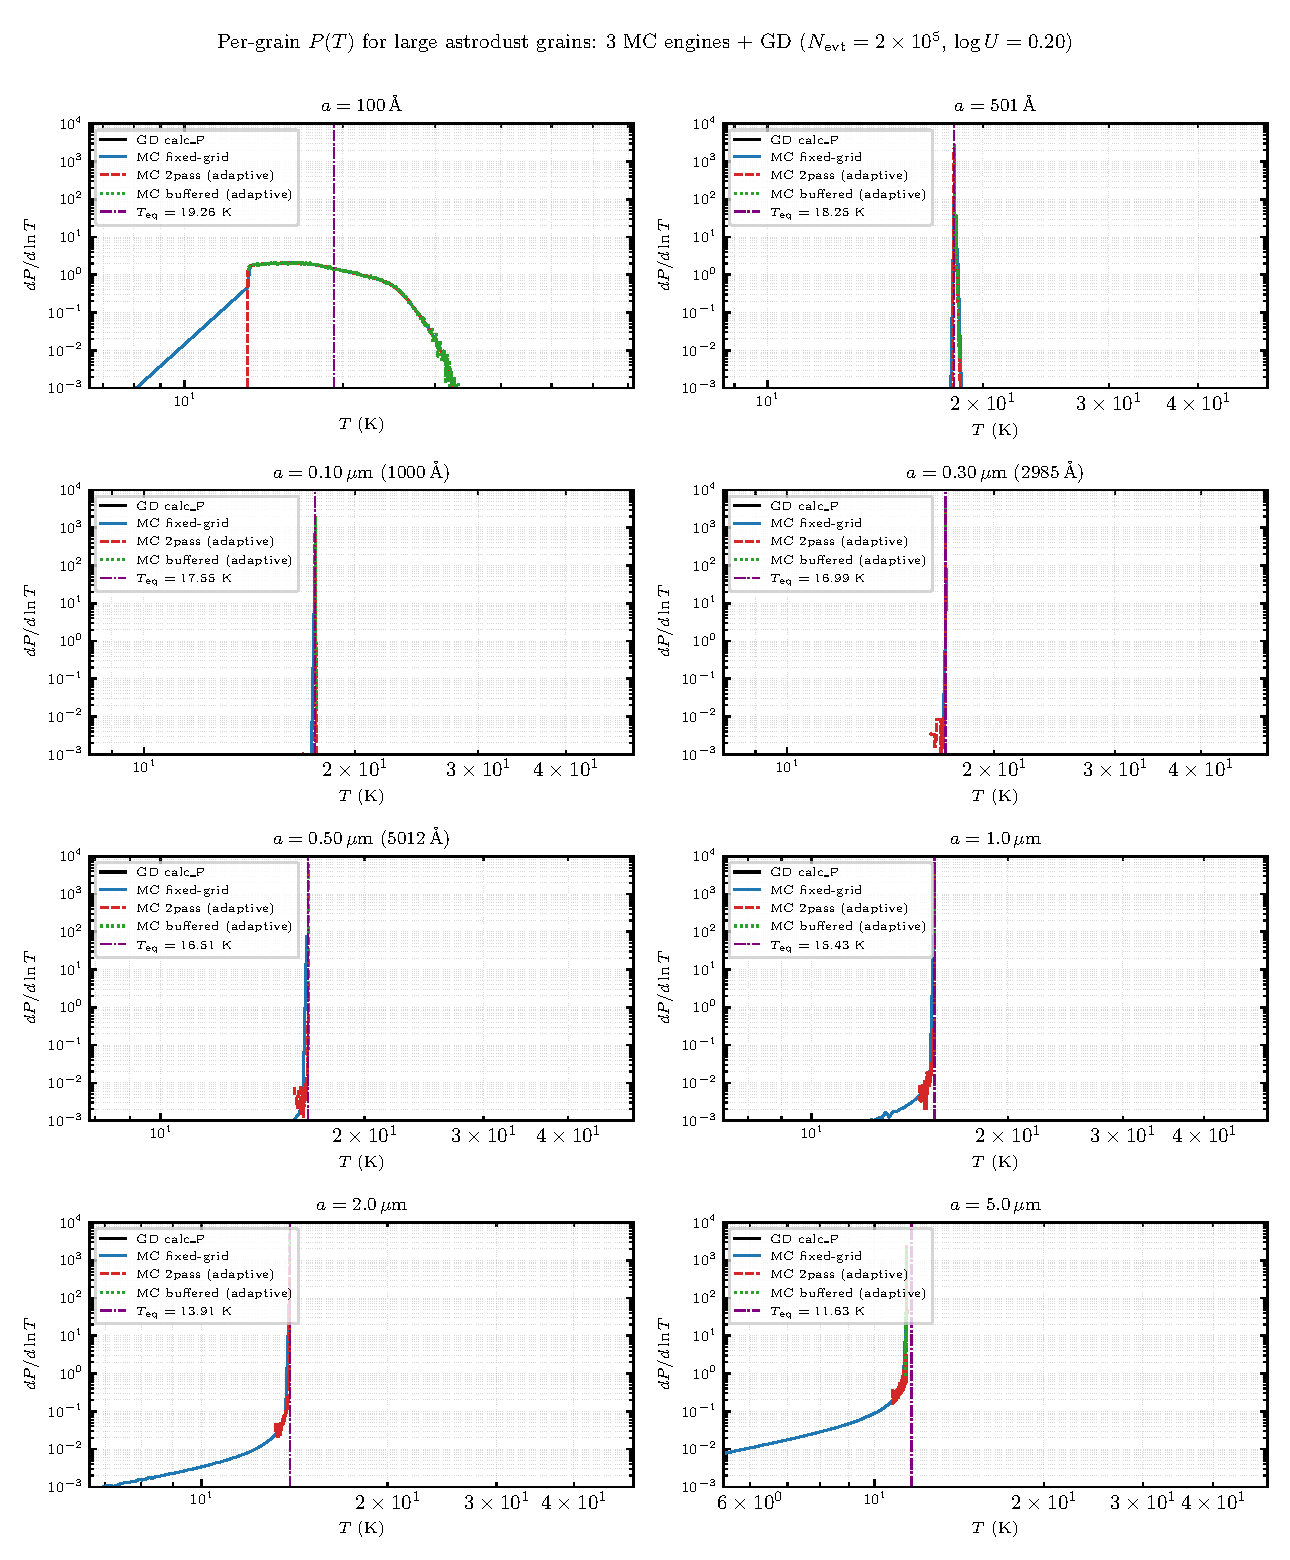
\includegraphics[width=\linewidth]{figs/pT_compare_large.pdf}
\caption{Single-grain $dP/d\ln T$ for large astrodust grains
  ($a\in\{100, 501, 1000\,\textrm{\AA}, 0.3, 0.5, 1, 2, 5\,\mu$m$\}$,
  Stage~2 enthalpy, Mathis ISRF at $\log U=0.20$, $N_{\rm evt}=2\times 10^5$).
  Purple vertical line: $\Teq$ from \texttt{calc\_Teq}. Black: GD
  \texttt{calc\_P}; blue: fixed-grid MC; red dashed: 2pass adaptive;
  green dotted: buffered adaptive. With the adaptive
  $\lambda_c(a)$ (\S\ref{sec:adaptive_lamc}) the MC trajectories
  hold tightly at $\Teq$ for every panel from $100$\,\AA{} to
  $5\,\mu$m; the trajectory collapse toward CMB seen with a static
  $\lambda_c=1000\,\mu$m is fully removed.}
\label{fig:pT_large}
\end{figure}

\bibliographystyle{plainnat}
\begin{thebibliography}{9}

\bibitem[Draine \& Anderson(1985)]{DraineAnderson1985}
Draine, B.~T., \& Anderson, N.\ 1985, ApJ, 292, 494,
``Temperature fluctuations and infrared emission from interstellar
grains''.

\bibitem[Draine(2011)]{DrainePIIM2011}
Draine, B.~T.\ 2011, \emph{Physics of the Interstellar and
Intergalactic Medium} (Princeton: Princeton University Press), Chap.\ 24.

\bibitem[Guhathakurta \& Draine(1989)]{GuhathakurtaDraine1989}
Guhathakurta, P., \& Draine, B.~T.\ 1989, ApJ, 345, 230,
``Temperature fluctuations in interstellar grains.\ I.\ Computational
method''.

\bibitem[Draine \& Li(2001)]{DraineLi2001}
Draine, B.~T., \& Li, A.\ 2001, ApJ, 551, 807,
``Infrared emission from interstellar dust.\ I.\ Stochastic heating
of small grains''.

\bibitem[Mattioda et al.(2005)]{Mattioda2005}
Mattioda, A.~L., Allamandola, L.~J., \& Hudgins, D.~M.\ 2005, ApJ,
629, 1188, ``The near-infrared spectrum of polycyclic aromatic
hydrocarbon cations''.

\bibitem[Draine(2016)]{Draine2016}
Draine, B.~T.\ 2016, ApJ, 831, 109, ``Graphite Revisited''.

\bibitem[Hensley \& Draine(2023)]{HensleyDraine2023}
Hensley, B.~S., \& Draine, B.~T.\ 2023, ApJ, 948, 55,
``The astrodust+PAH model''.

\end{thebibliography}
\end{document}
